\chapter{Esperimento e Risultati}\label{ch:chapter3}
\section{Introduzione al Progetto}
Prima di poter iniziare a mostare il progetto è necessario porre delle basi e limiti per quest'ultimo.
Per analizzare il problema del \textbf{Continual Learning} ci concentreremo su problemi di \textit{classificazione} che è un probelma tipico del \textit{Deep Learning}. La classificazione implica la previsione a quale classe appartiene un elemento. Alcuni classificatori sono binari, altri sono multi-classe, in grado di classificare un \textit{Item} in una delle diverse categorie. Noi  , quindi, ci andremo a concentrare sull'utilizzo di un classificatore \textit{multi-classe}.
\newline
La seconda limitazione riguarda l'approccio \textbf{\textit{Task Incremental}}. Il \textbf{\textit{Task Incremental}} corrisponde ad un approccio in cui i dati arrivano in sequenza di \textit{batches} e ogni
\textit{batch} corrisponde ad un \textit{Task}. Ad ogni\textit{Task} corrisponderà un nuovo insieme di \textit{labels} il cui numero dipenderà dalla quantità di quest'ultime(nel \textit{Dataset}) e dalla loro divisione. In altre parole, assumiamo  che per un dato \textit{Task}, tutti i dati diventino disponibili simultaneamente seguendo Il concetto di \textit{Training Offline}. Ciò consente un \textit{Training} per più epoche su tutti i suoi dati di addestramento, mescolati ripetutamente per garantire delle condizioni di 
\textit{i.i.d.}. È importante sottolineare che i dati appartenenti al  precedente o al futuro \textit{Task}
non saranno utilizzabili. Ottimizzare/Allenare per un nuovo \textit{Task} in questa configurazione si tradurrà nel \textit{\textbf{Catastrophic Forgetting}}, con significativi
cali sulle prestazioni relative ai vecchi \textit{Task}, salvo startegie specifiche siano adottate.
\newline 
A differenza della limitazione alla configurazione \textit{Multi-Head} utilizzata nel paper FARE LA CITAZIONE,
in questo elaborato proveremo a analizzare entrambe le configurazioni \textit{Multi-Head/single-Head}. Ciò corrispinde ai due approcci che abbiamo già intordotto nel primo capitolo: \textbf{Task-Agnostic/Task-Aware}. Nel caso di \textbf{Task-Agnostic} avremo una single \textit{Head} per tutti i \textit{Tasks} perchè non conosciamo su quale stiamo facendo \textit{Trainin/Testing}, mentre per \textbf{Task-Aware} avremo una \textit{Multi-Head} e selezioneremo l'\textit{Output} corrispondente a quello corrente.
\section{Pipeline}
Per simulare il processo di \textbf{Continual Learning} ho dovuto stabilire una \textit{Pipeline}che avrebbe dovuto seguire l'algoritmo. A seconda delle tipologie di approccio 
\textbf{Task-Agnostic/Task-Aware} avremo delle differenze all'interno della \textit{Pipeline} che analizzerò successivamente.
\newline
Per analizzare al meglio il problema del \textit{Catastrophic Forgetting}
ho deciso di dividere il dataset in 5 \textit{batches} ciascuno con i dati relativi relativi a due label, visto che \textit{CIFAR-10} ha 10 classi. Se avessi usato solamente due \textit{Tasks} avrei potuto ottnere risultati poco significativi per il progetto.
\newpage
La \textbf{\textit{Pipeline}} del processo è questa che segue:
\begin{enumerate}
    \item Creare \textit{Rete Neurale convoluzionale}  che farà da \textit{Backbone}
    \item Per ogni t in \textit{Tasks}:
    \begin{enumerate}
        \item Aggiungo un nuovo \textit{Classification Module} per il \textit{Task} corrente.
        \item \textit{SetTask} per selezionare l'\textit{output} corretto della rete a seconda di  \textit{Aware/Agnostic Training}. 
        \item Fare il \textit{Training} per il \textit{Task} t
        \item \textit{SetTask} per selezionare l'\textit{output} corretto della rete a seconda di  \textit{Aware/Agnostic Testing}.
        \item Fare \textit{Test} della \textit{Network} per il \textit{Task} t.
     \end{enumerate}
    \item Fare \textit{Test} della \textit{Network} per ogni \textit{Task} dopo l'ultimo \textit{Training}, selezionando \textit{Output} giusto per la tipologia di \textit{Testing}.
\end{enumerate}
\mathbf{2.b/2.d/3} sono le fasi che vengono influenzate dalla scelta della tipologia di \textit{Training7Testing-Agnostic/Aware}. Ciò consiste nel fatto che l'\textit{Output} della rete verrà modificato seguendo il paradigma \textit{Task-Aware/Task-Agnostic}, diventando unico per più \textit{Tasks} nel caso \textit{Agnostic} e unico per il \textit{Task} specifico per \textit{Aware}.\newline
Inoltre il processo della \textit{Pipeline} sarà il medesimo sia, al variare del numero di \textit{Tasks} che della formazione di quest'ultimi(\textit{Labels randomiche}).\newline
Avremo, quindi, 5 configurazioni diverse di Processi di cui 4 andranno a combinare \textit{Aware/Agnostic outputs} e una sarà relativa al \textit{Joint-Train}.\newline
Mostrerò i risultati ottenuti nelle quattro configurazioni tenendo presente come \textit{Upperbound} il valore della \textit{Accuracy} ottenuta dal \textit{Joint-Train}.
\newpage
\section{Esperimenti}
Quindi le configuazioni di nostro interesse saranno:
\begin{enumerate}
     \item \textbf{\textit{Joint-Training/Testing}}: Corrisponde sostanzialmente ad allenare e testare la rete su tutte le \textit{Labels} contemporaneamente. Sarà equivalente ad un unico \textit{Task} con tutti gli \textit{examples} del \textit{Dataset}
    
    \item \textbf{\textit{Task-Agnostic Training}/\textit{Task-Agnostic Testing}}: \textit{Training} con \textit{Output} per ogni \textit{Task}, \textit{Testing} con \textit{Output} per ogni \textit{Task}.  
    
    \item \textbf{ \textit{Task-Agnostic Training}/\textit{Task-Aware Testing}} : \textit{Training} con \textit{Output} per ogni \textit{Task}, \textit{Testing} con \textit{Output} per \textit{Task} specifico.
    
    \item \textbf{\textit{Task-Aware Training}/\textit{Task-Aware Testing}} : \textit{Training} con \textit{Output} per \textit{Task} specifico, \textit{Testing} con \textit{Output} per \textit{Task} specifico. 
    
    \item \textbf{\textit{Task-Aware Training}/\textit{Task-Agnostic Testing}}: \textit{Training} con \textit{Output} per \textit{Task} specifico, \textit{Testing} con \textit{Output} per ogni \textit{Task}  
\end{enumerate}
Per comprendere nel miglior modo i risultati andrò a rappresentare le \textit{accuracies} delle configuazioni in due grafici. Il primo sarà relativo al \textit{Task-Agnostic Training} riportando le \textit{accuracies} relative ai casi \textit{Aware/Agnostic} così da visualizzare le differenze, mentre il secondo avrà \textit{Task-Aware Training}. Entrambi i grafici saranno equiparati al valore \textit{Joint-Train} che rappresenterà l'\textit{Upperbound} per qualsiasi configurazione. \newline
Un altro valore importante da analizzare per comprendere al massimo il valore del \textit{Catastrophic Forgetting} è la differenza tra la media delle \textit{acuracies} dopo l'allenamento realitivo a ciascun \textit{Task} e quella dopo l'ultimo \textit{Task}. Questo valore ci fornisce il \textbf{\textit{Catastrophic Forgetting}} a cui siamo andati in contro grazie al \textit{Continual Learning}.
\newpage
\subsection{Joint-Training}
Prima di andare ad analizzare le varie configurazioni è necessario concentrarci sul \textbf{\textit{Joint-Training}}.
Il \textbf{\textit{Joint-Training}} corrisponde al generico procedimento di \textit{Training/Testing} che viene eseguito nel \textit{Visual Rcognition}.Ciò, consiste in un addestramento e \textit{testing} fatto sulla totalità degli esempi appartenenti ai \textit{batches} che compongono il \textit{Dataset} senza considerare la divisione in \textit{Tasks} violando, quindi, il paradigma del \textit{Continual Learning}. Questa \textit{Baseline} ci fornisce un \textit{UpperBound} per le \textit{accuracies} rilevate.
Il valore di \textit{accuracy} che abbiamo ottenuto dal nostro \textit{Joint-Training} è di \textit{\textbf{77.6}} è lo utilizzeremo come riferimento nei nostri grafici. 
\subsection{Agnotic-Training}
Qui di seguito riporto il Grafico con i risultati ottenuti sia per \textit{Agnostic} che \textit{Aware Training}: 
\begin{figure}[ht]
\centering
\caption{Agnostic Training}
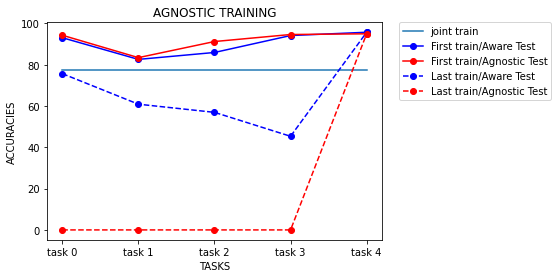
\includegraphics[width=\linewidth]{Agnostic_Agnostic-Aware.png}
\label{figure : Angostic_training}
\end{figure}
\newpage
Prima di analizzare il grafico  andiamo a considerare il paradigma l'\textit{Agnostic-Training} che consiste nel \textit{Training}
senza sapere di quale \textit{Task} ci stiamo occupando.
Ciò comporta che ad ogni \textit{Task} l'output della rete consisterà in tutti i moduli dei \textit{Tasks} fino a quello corrente concatenati nel metodo \textit{Forward}, questo perchè non possiamo selezionare l'\textit{output} relativo al \textit{Task} in esecuzione.
\newline
Dal grafico ~\ref{figure : Angostic_training}, che si trova a pagina precendete, possiamo notare vari aspetti interessanti sui risultati ottenuti. Prima di tutto, notiamo che i valori delle \textit{accuarcies} sui vari \textit{Tasks} calcolate dopo i rispettivi \textit{Training} ottengono valori molto elevati che superano persino il valore del \textit{Joint Train}. Questo è dovuto al numero minore di dati utilizzati rispetto al \textit{Dataset} completo e dal fatto che il \textit{Test} è effetuato subito  dopo il \textit{Training} del relativo \textit{Task}. Inoltre, da notare, come i due approcci di \textit{Testing} ottengano \textit{accuracies} quasi identiche, questo perchè la rete viene \textit{testata} subito dopo il \textit{train} relativo di conseguenza i pesi associati alla clasificazione sono molto precisi per entrambe le configurazioni, ottenendo risulati, per ciascun \textit{Task}, migliori anche del \textit{Joint Train} .
L'\textit{accuracy} calcolata sull'ultimo \textit{task}, naturalmente, avrà valore uguale per tutte e quattro le configurazioni, come si può nel grafico ~\ref{figure : Angostic_training} nel punto relativo a quest'ultimo.
\newline
Per quanto riguarda le \textit{accuracies} calcolate successivamente all'ultimo\textit{Training}, vediamo che otteniamo un calo drastico di precisione su ciasciun \textit{Task} escluso l'ultimo come abbiamo precedentemente notato. Questo è il fenomeno del \textbf{Catastrophic Forgetting}, introdotto nel \autoref{ch:chapter1}, che porta il \textit{modello} a dimenticare tutti i \textit{weight} relativi ai \textit{Tasks} precedenti.
In Particolare nella configurazione Aware otteniamo dei valori migliori dati dall'output più preciso e specifico per il relativo \textit{Task}, ottenuto selezionando la \textit{Classification Head} realtiva a quest'ultimo. Per quanto riguarda la configurazione di \textit{Agnostic Testing}, otteniamo un valore molto alto per l'ultimo \textit{Task} mentre per i 4 precedenti l'\textit{accuracy} va a 0. Queto fenomeno prende il nome di 
\textit{\textbf{Task Recency Bias}}. Si tratta di un fenomeno che consiste nel fatto che la \textit{rete} tenda a ricordare e a prevedere meglio dati su cui è stato fatto per ultimo il \textit{Training} portando a dimenticare totalmente i \textit{Tasks} precedenti, come viene descritto in \textbf{FARE CITAZIONE AL PAPER}. Questo risultato è rincondotto all'utilizzo di \textit{CrossEntropyLoss}  che aumenta il valore della probabibiltà relativa alla classe corretta e abbassa quella relativa alla classe non corretta all'interno della distribuzione di probabilità, siccome grazie al \textit{SoftMax} la somma dei valori deve essere uguale a uno. Ad ogni esempio del batch del \textit{Task} corrente butta giù la probabilità delle classi appartenenti a quelli precedenti andando incontro al \textbf{Catastrophic Forgetting}.
\newline
Per questo motivo è interessante valutare le medie delle \textit{accuracies} per analizzare l'occorrere del \textbf{Catastrophic Forgetting} nelle varie configurazioni.
Qui di seguito i valori delle accuracy riporatet in due tabelle, una per tipologia di \textit{Testing}.
\begin{table}[!htb]
\begin{minipage}{.5\linewidth}
    \centering

    \label{tab:Agnostic-Agnostic }

    \medskip

\begin{tabular}{l*{6}{c}r}
Tasks   & First Train & Last Train\\
\hline
   Task 0      &     94.30      &      0.0\\
   Task 1      &     83.45      &      0.0\\
   Task 2      &     91.25      &      0.0\\
   Task 3      &     94.65      &      0.0\\
   Task 4      &     95.00      &      95.00\\
\end{tabular}
\caption{Agnostic-Agnostic}
\label{tab:Agnostic-Agnostic}
\end{minipage}\hfill
\begin{minipage}{.5\linewidth}
    \centering

    \label{tab:Agnostic-Aware}

    \medskip

\begin{tabular}{l*{6}{c}r}
Tasks   & First Train  & Last Train\\
\hline
   Task 0      &     93.10      &      75.70\\
   Task 1      &     82.60      &      60.90\\
   Task 2      &     85.95      &      56.95\\
   Task 3      &     94.15      &      45.35\\
   Task 4      &     95.75      &      95.75\\
\end{tabular}
\caption{Agnostic-Aware}
\label{tab:Agnostic-Aware}
\end{minipage}
\end{table}
\newline
Nelle tabelle~\ref{tab:Agnostic-Agnostic} e~\ref{tab:Agnostic-Aware} notiamo, come avevamo già fatto nel grafico in figura ~\ref{figure : Angostic_training} a pagina ~\pageref{figure : Angostic_training}, che l'\textit{accuracy} della configurazione \textit{Agnostic-Agnostic} è peggiore rispetto a quella di \textit{Agnostic-Aware} ma per valutare la differenza di valori, ma soprattutto il \textit{Forgetting}, calcoliamo la media i quest'ultimi.
\newline
Facendo le medie otteniamo i seguenti valori:
\begin{itemize}
    \item Tabella~\ref{tab:Agnostic-Agnostic}: Abbiamo una \textit{accuracy} iniziale di 91.73\% e finale del 19.0\%, quindi otteniamo un decremento del 72.71\%.
    \item Tabella~\ref{tab:Agnostic-Aware}: Abbiamo una \textit{accuracy} iniziale di 90.30\% e finale del 66.92\%, quindi otteniamo un decremento del 23.38\%.
\end{itemize}
Notiamo che la media dell'\textit{accuracy} del \textit{Task Agnostic} e \textit{Task Aware Testing} sono entrambe inferiori dell'\textit{Upperbound} rappresentato dal \textit{Joint-Train}, confermando ciò che si poteva notare già a livello grafico nell'immagine~\ref{figure : Angostic_training}.
Il decremento della \textit{accuracy} ci serve a valutare l'entità del \textit{Catastrophic Forgetting} a cui siamo andati incontro.
\newline
Questo valore inoltre ci conferma il \textit{forgetting} molto elevato che abbiamo ottenuto sui \textit{Tasks} precedenti all'ultimo  utilizzando la configurazione \textit{Agnostic-Agnostic}. Vedremo successivamente una soluzione naive al problema del \textit{Task Recency Bias}(che colpisce in minor modo la configurazione \textit{Agnostic-Aware}), basato sull'approccio \textit{Replay Based Methods}.
\newline
In generale il decremento di \textit{accuracy} per entrambe le configurazioni utilizzate in questo paragrafo, è elevato anche se con entità diverse. Inoltre la distanza di \textit{accuracy} in media dal valore ottenuto con il \textit{Joint-Train} assume un valore del 10,68\%, per la configurazione \textit{Agnostic-Aware}, 58,60\% per \textit{Agnostic-Agnostic}. Questo ci fa comprendere l'entità del \textit{drop} di \textit{accuracy} a cui si può andare incontro adottando una divisione in \textit{Tasks} dovuto al \textit{catastrophic forgetting}.
\subsection{Aware-training}
In queta sezione ci concentriamo su altre due configurazioni\textit{Task-Aware} per il \textit{Training} introdotte già a \textit{pag.} 14.
A differenza della configurazione \textit{Task-Aware} possiamo selezionare la \textit{Classification Head} relativa al \textit{Task} corrrente, di conseguenza il \textit{Training} per ognuno di essi sarà eseguito con un \textit{output} di soli due valori modificando quindi l'aggiornamento dei parametri della \textit{Rete}.\newline
Riportiamo qui di seguito il grafico che rappresenta le accuracy:
\begin{figure}[ht]
\centering
\caption{Agnostic Training}
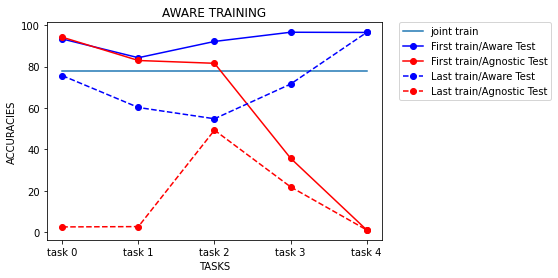
\includegraphics[width=\linewidth]{Aware_Agnostic-Aware.png}
\label{figure : Aware_Training}
\end{figure}
\newline
Dalla figura ~\ref{figure : Aware_Training} possiamo notare che l'andamento generale delle accuracy segue, in linea generale, quello della figura ~\ref{figure : Angostic_training} a pagina 15.
Di conseguenza abbiamo che l'\textit{accuracy} su un \textit{Task} calcolata subito dopo il corrispondente addestramento ha un valore molto buono, che in media è addirittura superiore al \textit{Joint Train}, sia per \textit{Aware} che \textit{Agnostic Test}. Inoltre abbiamo che l'accuracy sull'ultimo \textit{Task} ha lo stesso valore per tutti i casi riportati, tranne uno \textit{Aware-Agnostic}. Si può notare che l'\textit{accuracy} calcolata sull'ultimo \textit{Task} a seconda della tipologia assume dei valori diversi.
In particolare la configurazione \textit{Agnostic Test} notiamo che l'accuracy subito dopo il \textit{Training} assume un valore sempre minore fino all'ultimo \textit{Task} in cui è quasi nulla. Questo risultato è ottenuto perchè durante la fase \textit{Train} utilizziamo la \textit{classification head} specifica del \textit{Task} mentre nella fase di \textit{Testing} utilizziamo un \textit{output} unico per tutti \textit{Tasks} fino a quello corrente.
Adesso mostriamo di seguito la tabella con le accuracy ottenute per poter capire il \textit{forgetting} ottenuto e comparare i risultati con l' \textit{Agnostic Train}:
\begin{table}[!htb]
\begin{minipage}{.5\linewidth}
    \centering

    \label{tab:Aware-Agnostic }

    \medskip

\begin{tabular}{l*{6}{c}r}
Tasks   & First Train & Last Train\\
\hline
   Task 0      &     94.15      &       2.50\\
   Task 1      &     82.90      &       2.65\\
   Task 2      &     81.55      &      49.25\\
   Task 3      &     35.70      &      21.85\\
   Task 4      &      1.05      &       1.05\\
\end{tabular}
\caption{Aware-Agnostic}
\label{tab:Aware-Agnostic}
\end{minipage}\hfill
\begin{minipage}{.5\linewidth}
    \centering

    \label{tab:Aware-Aware}

    \medskip

\begin{tabular}{l*{6}{c}r}
Tasks   & First Train  & Last Train\\
\hline
   Task 0      &     93.30      &      75.60\\
   Task 1      &     84.25      &      60.20\\
   Task 2      &     92.10      &      54.75\\
   Task 3      &     96.55      &      71.50\\
   Task 4      &     96.45      &      96.45\\
\end{tabular}
\caption{Aware-Aware}
\label{tab:Aware-Aware}
\end{minipage}
\end{table}
\newline
Nelle tabelle ~\ref{tab:Aware-Agnostic} e ~\ref{tab:Aware-Aware} notiamo subito che la accuracy rilevata nel caso di \textit{Aware Testing} è migliore, ma consideriamo adesso le medie delle \textit{accuracies} e il \textit{Forgetting} ottenuto.
\begin{itemize}
    \item Tabella~\ref{tab:Aware-Agnostic}: Abbiamo una \textit{accuracy} iniziale di 59.07\% e finale del 15.45\%, quindi otteniamo un decremento del 43.61\%.
    \item Tabella~\ref{tab:Aware-Aware}: Abbiamo una \textit{accuracy} iniziale di 92.53\% e finale del 71.7\%, quindi otteniamo un decremento del 20.83\%.
\end{itemize}
La prima cosa che notiamo è che l'accuracy iniziale della configurazione \textit{Agnostic-Agnostic} ha ottenuto un valore in media molto minore rispetto alle altre causato dall'\textit{Agnostic Testing}.
L'accuracy ottenuta nel caso \textit{Aware-Aware} è il miglior risultato e si avvicina a quella del \textit{Joint-Train} con uno scarto del 5,9\%. Mentre nel caso della Tabella ~\ref{tab:Aware-Agnostic} l'\textit{Accuracy} ottenuta rappresenta il \textit{Lower-Bound} dei risultati con uno scarto dal \textit{Joint-Train} del 62,15\%. 
\section{Soluzione Naïve}
In questa sezione andiamo ad proporre una soluzione con un \textit{naïve} al probelma del \textit{Catastrophic Forgetting}. Esistono tre famiglie di soluzioni al problema del \textit{Continual Learning}:
\begin{itemize}
    \item \textit{Replay methods}
    \item \textit{Regularization-based methods}
    \item\textit{Parameter isolation methods}
\end{itemize}
In questa sezione ci soffermeremo su una soluzione \textit{Naïve} dellla famiglia dei \textit{\textbf{Replay methods}}. Questo approccio consiste nel memorizzare i campioni o generare \textit{pseudo-campioni} con un modello generativo appartenenti ai \textit{Tasks} precedenti. Questi esempi  vengono riutilizzati durante l'apprendimento di un nuovo \textit{Task} per alleviare il \textit{Forgetting}.\newline
Il problema principale dei \textit{Replay methods} risiede nella memoria, salvando esempi dai \textit{Task} precendeti la memori necessaria a ciascun \textit{Task} sarà sempre maggiore. Ciò può esser ovviato utiizzando un limite di esempi possibili dai precedenti \textit{Tasks} ottenendo però una perdita di generalizzazione del rispettivo \textit{Task}.
PARLARE IN BREVE DEI METODI GEM E ICARL E SUCCESSIVAMENTE DELLA SCELTA NAIVE